
\documentclass[conference]{IEEEtran}

% ================= PACKAGES =================
\usepackage[T1]{fontenc}
\usepackage{cite}
\usepackage{graphicx}
\usepackage{url}
\usepackage{amsmath}
\usepackage{array}
\usepackage{booktabs}
\usepackage{tikz}
\usetikzlibrary{
    arrows.meta,
    positioning,
    shapes.geometric,
    fit,
    backgrounds,
    calc
}

% ================= TITLE =================
\title{KernelX: Design and Implementation of a Modular Educational Operating System Kernel}

\author{
\IEEEauthorblockN{Chethana Sri}
\IEEEauthorblockA{
Department of Computer Technology\\
Madras Institute of Technology, Anna University\\
Chennai, India
}
}

\begin{document}

\maketitle

% ================= ABSTRACT =================
\begin{abstract}
This paper presents KernelX, an educational operating-system
kernel project developed to explore low-level system software
through a bootable x86 kernel. The project incorporates a bootable
kernel foundation, a Virtual File System (VFS), an in-memory
RAMFS backend, TAR/USTAR archive handling for initial filesystem
content, filesystem-related kernel interfaces, and a kernel-resident
command shell. Development was performed in a Windows/WSL2
environment, with the image subsequently exercised in QEMU.
Reported validation includes host-side VFS and RAMFS tests,
a nested USTAR test, successful ISO generation and QEMU boot,
and a Phase 7 test run reported as 16 passing tests. This paper
describes the architecture, implementation approach, validation
results, and limitations of KernelX as an educational kernel
prototype.
\end{abstract}

\begin{IEEEkeywords}
Operating Systems, Kernel Development, Virtual File System,
RAMFS, TAR, USTAR, System Calls, x86 Architecture, QEMU.
\end{IEEEkeywords}

% ================= I. INTRODUCTION =================
\section{Introduction}

An operating-system kernel manages the interface between
hardware and software. It provides mechanisms through which
software components interact with processor facilities, memory,
devices, and storage. Kernel development provides practical
insight into bootstrapping, memory management, filesystem
abstractions, and command interfaces \cite{tanenbaum,stallings}.

KernelX is a learning-oriented operating-system kernel project
developed incrementally. The project includes boot and kernel
foundations, a Virtual File System (VFS), RAM-backed filesystem
support, TAR/USTAR archive handling, filesystem-related kernel
interfaces, and a kernel-resident shell.

The primary objective is to demonstrate modular kernel
organization and the integration of filesystem components
within a bootable x86 environment.

\subsection{Research Objectives}

The objectives of KernelX are:

\begin{itemize}
    \item Establish a bootable x86 kernel foundation.
    \item Implement a Virtual File System abstraction.
    \item Provide an in-memory RAMFS backend.
    \item Support TAR/USTAR archive handling for initial files.
    \item Expose filesystem operations through kernel interfaces.
    \item Provide a kernel-resident command shell.
    \item Validate selected components through automated tests
    and QEMU execution.
\end{itemize}

\subsection{Scope}

The reported shell is kernel-resident and is not an independently
loaded Ring 3 process. The available project record does not
establish a complete scheduler, user-mode process model,
network stack, persistent block-device filesystem, or
production-grade security boundary.

% ================= II. RELATED WORK =================
\section{Background and Related Work}

\subsection{x86 System Architecture}

Intel's Software Developer's Manual describes processor
operation, memory management, interrupts, exceptions, and
system-programming facilities required for x86 kernel
development \cite{intel}.

The Global Descriptor Table and Interrupt Descriptor Table
are important architectural structures used in x86 system
programming \cite{gdt,idt}.

\subsection{Bootloaders and Executable Formats}

The GNU GRUB Multiboot2 specification defines a standardized
interface between a bootloader and a kernel image \cite{multiboot}.

The Executable and Linking Format (ELF) specification describes
the structure of executable and object files used by toolchains
and loaders \cite{elf}.

\subsection{Virtual File Systems}

A Virtual File System provides a common interface between
filesystem consumers and concrete filesystem implementations.
Linux kernel documentation describes the VFS architecture
and its filesystem objects and operations \cite{vfs}.

This abstraction allows filesystem operations to remain
independent of the underlying storage implementation.

\subsection{Memory-Based Filesystems}

RAM-based filesystems provide temporary storage using system
memory. Linux documentation describes ramfs, rootfs, and
initramfs mechanisms \cite{initramfs}.

KernelX uses a RAMFS backend and reports TAR/USTAR archive
handling for initial filesystem content. These archive
mechanisms should not be confused with Linux's cpio-based
initramfs format.

\subsection{Virtualization and Testing}

QEMU provides machine emulation for executing and debugging
operating-system images \cite{qemu}. Emulator-based testing
allows kernel developers to observe boot behavior and
validate integration without requiring dedicated hardware.

% ================= III. PROBLEM STATEMENT =================
\section{Problem Statement}

Early kernel projects often develop boot code, filesystem
functionality, storage backends, and command interfaces as
separate components.

Without clear subsystem boundaries, filesystem consumers
can become tightly coupled to a particular storage
implementation. Testing may also require a complete machine
boot for every modification.

KernelX addresses this educational engineering problem by
organizing filesystem functionality around a VFS abstraction,
a RAMFS backend, archive-provided initial content, and a
kernel command interface.

The research focus is the modular organization and integration
of these components in a bootable educational kernel.

% ================= IV. SYSTEM ARCHITECTURE =================
\section{System Architecture}

KernelX follows a modular architecture consisting of a boot
environment, kernel initialization, kernel core subsystems,
filesystem components, and a kernel console interface.

The architecture separates filesystem abstraction from its
backend implementation and provides an integrated command
interface for interacting with the kernel.

\subsection{Architectural Diagram}

Fig.~\ref{fig:architecture} illustrates the overall architecture
of KernelX.

\begin{figure*}[!t]
\centering

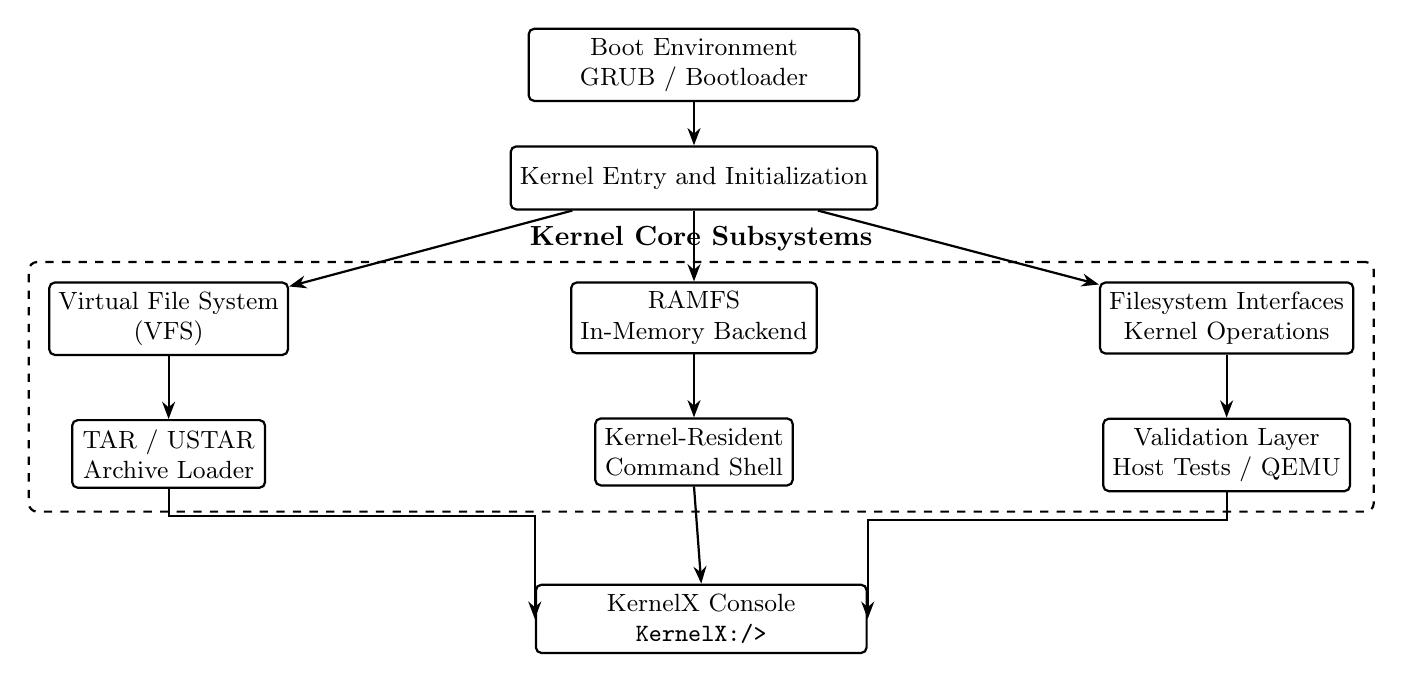
\begin{tikzpicture}[
    font=\small,
    block/.style={
        draw=black,
        rectangle,
        rounded corners=2pt,
        minimum width=3.0cm,
        minimum height=0.8cm,
        align=center,
        thick
    },
    subblock/.style={
        draw=black,
        rectangle,
        rounded corners=2pt,
        minimum width=2.45cm,
        minimum height=0.85cm,
        align=center,
        thick
    },
    arrow/.style={
        -{Stealth[length=2.2mm]},
        thick
    },
    dashedbox/.style={
        draw=black,
        dashed,
        rounded corners=3pt,
        thick,
        inner sep=7pt
    }
]

% Boot stage
\node[block, minimum width=4.2cm] (boot)
{Boot Environment\\GRUB / Bootloader};

\node[block, below=0.55cm of boot, minimum width=4.2cm] (entry)
{Kernel Entry and Initialization};

% Kernel core boundary
\node[subblock, below left=0.9cm and 2.8cm of entry] (vfs)
{Virtual File System\\(VFS)};

\node[subblock, below=0.9cm of entry] (ramfs)
{RAMFS\\In-Memory Backend};

\node[subblock, below right=0.9cm and 2.8cm of entry] (syscall)
{Filesystem Interfaces\\Kernel Operations};

\node[subblock, below=0.8cm of vfs] (archive)
{TAR / USTAR\\Archive Loader};

\node[subblock, below=0.8cm of ramfs] (shell)
{Kernel-Resident\\Command Shell};

\node[subblock, below=0.8cm of syscall] (validation)
{Validation Layer\\Host Tests / QEMU};

% Boundary
\begin{scope}[on background layer]
\node[dashedbox,
    fit=(vfs)(ramfs)(syscall)(archive)(shell)(validation),
    label={[font=\bfseries]above:Kernel Core Subsystems}
] (core) {};
\end{scope}

% Console
\node[block, below=0.9cm of core, minimum width=4.2cm] (console)
{KernelX Console\\\texttt{KernelX:/>}};

% Connections
\draw[arrow] (boot) -- (entry);

\draw[arrow] (entry) -- (vfs);
\draw[arrow] (entry) -- (ramfs);
\draw[arrow] (entry) -- (syscall);

\draw[arrow] (vfs) -- (archive);
\draw[arrow] (ramfs) -- (shell);
\draw[arrow] (syscall) -- (validation);

\draw[arrow] (archive.south) -- ++(0,-0.35) -| (console.west);
\draw[arrow] (shell.south) -- (console.north);
\draw[arrow] (validation.south) -- ++(0,-0.35) -| (console.east);

\end{tikzpicture}

\caption{Modular architecture of the KernelX educational operating system kernel.}
\label{fig:architecture}

\end{figure*}

\subsection{Boot and Initialization}

The boot environment loads the kernel image and transfers
control to the kernel entry point. Kernel initialization
establishes the initial execution environment before the
kernel subsystems become available.

\subsection{Virtual File System}

The VFS provides a common filesystem-facing abstraction.
It separates filesystem consumers from backend-specific
implementation details.

\subsection{RAMFS Backend}

RAMFS provides an in-memory filesystem backend. It allows
filesystem operations to be performed without requiring
physical storage devices.

\subsection{TAR/USTAR Archive Loader}

KernelX includes handling for TAR/USTAR archive structures
as a source of initial filesystem content. The project
history reports a passing nested USTAR test.

\subsection{Filesystem Interfaces and Shell}

Filesystem-related kernel interfaces connect filesystem
functionality to the shell and other kernel components.

The project includes a kernel-resident command shell that
provides an interactive interface through the reported
\texttt{KernelX:/>} prompt.

% ================= V. IMPLEMENTATION =================
\section{Implemented Components}

\subsection{Boot and Kernel Foundations}

The project record reports successful C compilation and
linking of a 32-bit ELF kernel, followed by successful ISO
generation and QEMU boot.

\subsection{Virtual File System and RAMFS}

VFS provides a common filesystem-facing abstraction.
RAMFS provides an in-memory backend that permits filesystem
operations without physical storage.

\subsection{TAR/USTAR Archive Handling}

KernelX handles TAR/USTAR archive structures as a source
of initial filesystem content. A nested USTAR test was
reported as passing.

\subsection{Filesystem Interfaces and Shell}

Filesystem-related kernel interfaces connect functionality
to the shell and other kernel components. The shell is
kernel-resident and is not a separate Ring 3 application.

% ================= VI. METHODOLOGY =================
\section{Development and Validation}

Development was carried out in a Windows environment using
WSL2. The workflow involved compiling C source files, linking
the kernel image, preparing a bootable ISO, launching the
image in QEMU, and running tests for filesystem components.

Host-side tests provide a faster feedback loop for isolated
logic, while QEMU checks whether the integrated image reaches
the expected boot and console state.

Reported outcomes include:

\begin{itemize}
    \item Successful C compilation and 32-bit ELF linking.
    \item Passing host-side VFS tests.
    \item Passing host-side RAMFS tests.
    \item Passing nested USTAR test.
    \item Successful ISO generation and QEMU boot.
    \item Phase 7 test output reporting 16 passing tests.
\end{itemize}

These are project-reported outcomes and are not independent
certification results.

% ================= VII. RESULTS =================
\section{Results}

Table~\ref{tab:results} summarizes the reported validation
activities.

\begin{table}[!t]
\centering
\caption{Reported Validation Results}
\label{tab:results}

\begin{tabular}{|p{0.62\columnwidth}|c|}
\hline
\textbf{Validation Activity} & \textbf{Outcome}\\
\hline
C compilation and ELF linking & Successful\\
\hline
VFS host tests & Passed\\
\hline
RAMFS host tests & Passed\\
\hline
Nested USTAR test & Passed\\
\hline
ISO generation and QEMU boot & Successful\\
\hline
Phase 7 test suite & 16 passed\\
\hline
\end{tabular}
\end{table}

The available results indicate that selected build, filesystem,
archive, and boot workflows operated in the reported
development setup.

% ================= VIII. DISCUSSION =================
\section{Discussion}

The architecture follows a modular progression. Boot and
kernel initialization establish the execution environment;
VFS separates filesystem consumers from backend details;
RAMFS supplies an initial backend; archive handling provides
test content; and the shell provides a way to exercise
kernel functionality.

The distinction between a kernel-resident shell and a
user-space shell is important. A command prompt alone does
not demonstrate privilege separation, process isolation,
or a complete system-call transition.

Similarly, a RAMFS implementation does not imply persistent
disk storage.

% ================= IX. LIMITATIONS =================
\section{Limitations and Future Work}

The available project record does not establish a complete
user-mode process model, scheduler, Ring 3 shell,
virtual-memory isolation, comprehensive device-driver
framework, persistent disk filesystem, networking stack,
or production security boundary.

Future work includes:

\begin{itemize}
    \item Implementing a verified user-mode transition.
    \item Developing a system-call ABI.
    \item Introducing process and thread scheduling.
    \item Implementing paging and memory protection.
    \item Extending interrupt and exception handling.
    \item Supporting persistent block-device storage.
    \item Adding filesystem permissions and broader testing.
\end{itemize}

% ================= X. CONCLUSION =================
\section{Conclusion}

This paper presented KernelX as an educational x86 operating
system kernel project with reported boot foundations, a VFS
abstraction, RAMFS, TAR/USTAR archive handling, filesystem-related
kernel interfaces, and a kernel-resident shell.

The project history reports passing filesystem and archive
tests, successful ISO generation and QEMU boot, and a Phase 7
result of 16 passing tests.

Further implementation and validation are required before
describing KernelX as a complete general-purpose operating system.

% ================= REFERENCES =================
\begin{thebibliography}{25}

\bibitem{intel}
Intel Corporation,
\emph{Intel 64 and IA-32 Architectures Software Developer's Manual}.
Available: \url{https://www.intel.com/content/www/us/en/developer/articles/technical/intel-sdm.html}.

\bibitem{multiboot}
Free Software Foundation,
\emph{Multiboot2 Specification, Version 2.0}.
Available: \url{https://www.gnu.org/software/grub/manual/multiboot2/multiboot.html}.

\bibitem{elf}
Tool Interface Standards,
\emph{Executable and Linking Format (ELF) Specification}.
Available: \url{https://refspecs.linuxfoundation.org/elf/elf.pdf}.

\bibitem{vfs}
Linux Kernel Documentation,
\emph{Overview of the Linux Virtual File System}.
Available: \url{https://docs.kernel.org/filesystems/vfs.html}.

\bibitem{initramfs}
Linux Kernel Documentation,
\emph{Ramfs, Rootfs and Initramfs}.
Available: \url{https://docs.kernel.org/filesystems/ramfs-rootfs-initramfs.html}.

\bibitem{qemu}
QEMU Project,
\emph{QEMU System Emulation User's Guide}.
Available: \url{https://www.qemu.org/docs/master/system/introduction.html}.

\bibitem{tanenbaum}
A. S. Tanenbaum and H. Bos,
\emph{Modern Operating Systems},
4th ed. Pearson, 2015.

\bibitem{stallings}
W. Stallings,
\emph{Operating Systems: Internals and Design Principles},
9th ed. Pearson, 2018.

\bibitem{love}
R. Love,
\emph{Linux Kernel Development},
3rd ed. Addison-Wesley, 2010.

\bibitem{bovet}
D. P. Bovet and M. Cesati,
\emph{Understanding the Linux Kernel},
3rd ed. O'Reilly Media, 2005.

\bibitem{osdev}
OSDev Wiki,
\emph{Bare Bones}.
Available: \url{https://wiki.osdev.org/Barebones}.

\bibitem{higherhalf}
OSDev Wiki,
\emph{Higher Half Kernel}.
Available: \url{https://wiki.osdev.org/Higher_Half_Kernel}.

\bibitem{paging}
OSDev Wiki,
\emph{Setting Up Paging}.
Available: \url{https://wiki.osdev.org/Setting_Up_Paging}.

\bibitem{idt}
OSDev Wiki,
\emph{Interrupt Descriptor Table}.
Available: \url{https://wiki.osdev.org/Interrupt_Descriptor_Table}.

\bibitem{grub}
GNU Project,
\emph{GNU GRUB Manual}.
Available: \url{https://www.gnu.org/software/grub/manual/grub/grub.html}.

\bibitem{gdt}
OSDev Wiki,
\emph{Global Descriptor Table}.
Available: \url{https://wiki.osdev.org/Global_Descriptor_Table}.

\bibitem{pit}
OSDev Wiki,
\emph{Programmable Interval Timer}.
Available: \url{https://wiki.osdev.org/Programmable_Interval_Timer}.

\bibitem{ata}
OSDev Wiki,
\emph{ATA PIO Mode}.
Available: \url{https://wiki.osdev.org/ATA_PIO_Mode}.

\bibitem{drepper}
U. Drepper,
\emph{How To Write Shared Libraries}.
Red Hat, 2002.

\bibitem{dennis}
J. B. Dennis and E. C. Van Horn,
``Programming Semantics for Multiprogrammed Computations,''
\emph{Communications of the ACM},
vol. 9, no. 3, pp. 143--155, 1966.

\bibitem{ritchie}
D. M. Ritchie and K. Thompson,
``The UNIX Time-Sharing System,''
\emph{Communications of the ACM},
vol. 17, no. 7, pp. 365--375, 1974.

\bibitem{tar}
J. Gilmore,
\emph{GNU Tar Manual}.
Available: \url{https://www.gnu.org/software/tar/manual/}.

\bibitem{posix}
IEEE and The Open Group,
\emph{The Open Group Base Specifications, POSIX}.
Available: \url{https://pubs.opengroup.org/onlinepubs/9699919799/}.

\bibitem{ostep}
R. Arpaci-Dusseau and A. Arpaci-Dusseau,
\emph{Operating Systems: Three Easy Pieces}.
Available: \url{https://pages.cs.wisc.edu/~remzi/OSTEP/}.

\bibitem{intelopt}
Intel Corporation,
\emph{Intel 64 and IA-32 Architectures Optimization Reference Manual}.
Available: \url{https://www.intel.com/content/www/us/en/developer/articles/technical/intel-sdm.html}.

\end{thebibliography}

\end{document}
